\chapter{Novel Description of the Wobbling Bands}
\label{chapter-7-novel}

In this chapter, a unique picture for the description of wobbling bands will be developed. This formalism is based on the $\mathbf{W_1}$ approach, which was systematically treated in the previous chapter, showing its validity through the comparison with the experimental measurements. It will also follow a semi-classical picture, and the main goal is to fully describe the wobbling spectra of nuclei in which admixtures of positive- and negative-parity bands occur. Consequently, the new method will be tested on $^{163}$Lu, since the fourth wobbling band (TSD4) consists of states $I^\pi$ where $\pi=-1$.

The work that will be depicted here is in fact based on three papers published by the team. Indeed, in Ref. \cite{poenaru2021parity}, the key concept standing behind this interpretation were pointed out and new results concerning the excitation energies were obtained, while in Refs. \cite{poenaru2021extensive1,poenaru2021extensive2}, the authors took the model even further to calculate other quantities such as Routhians, rotational frequencies, and wobbling energies. Moreover, the geometrical interpretation of the \emph{Classical Energy Function} (CEF) was extensively studied in terms of its behavior near the critical points, meaning that an interest is devoted in finding stable/unstable wobbling motion. On top of that, graphical representations with two constants of motion, i.e., the total energy and the total angular momentum are realized for this nucleus, pointing out the \emph{allowed} classical trajectories of the system. As it will be shown, the information retrieved from these figures proves to be an efficient way of understanding this collective phenomenon unique to triaxial nuclei. The classical study of the wobbling picture for $^{163}$Lu in \cite{poenaru2021extensive2} is a remarking characteristic of the model, as the alternative treatments from the literature are based on quantal pictures that do not have a clear and `easy-to-grasp' physical meaning regarding the system dynamics. In addition, the study of collective motion in terms of stability diagrams in relation to a classical set of coordinates is another first within literature.

This chapter will be structured as follows: $1)$ a part that will cover the energy spectrum of $^{163}$Lu (as per Ref. \cite{poenaru2021extensive1}) and $2)$ a part that will be focused on the classical view of the stability and trajectories (according to the investigations from Ref. \cite{poenaru2021extensive2}). More concisely, part $1)$ will cover:
\begin{itemize}
    \item introduction of \emph{Signature Partner} + \emph{Parity Partner Bands}
    \item new analytical formula for the wobbling spectrum for $^{163}$Lu
    \item numerical calculations for the excitation energies
    \item interpretation of the free parameters in relation to other studies
\end{itemize}
while part $2)$ will be focused on:
\begin{itemize}
    \item formalism of the energy function employed in the context of Parity Partner Bands
    \item analytical expressions for CEF in the critical regions
    \item contour plots are constructed with the obtained CEF(s)
    \item \emph{nuclear trajectories} (i.e., intersection curves of the energy and angular momentum) 
\end{itemize}

Obviously, for both parts some general discussions will be made, emphasizing the main results that emerge from the considerations.

\section{Parity Partner Bands}
\label{parity-partners-renormalizaion}

Recalling the main features that were adopted in the $\mathbf{W_1}$ formalism for the odd$-A$ $^{163}$Lu nucleus, all its wobbling properties were described through the TDVE (Eq. \ref{tdve-approach-w1}), which was used in the bands TSD1-2 and TSD4, respectively. The TSD3 band was the one-wobbling-phonon band built as an excitation on top of TSD2. The bands TSD1-2 were considered Signature Partner Bands, where the former has the favored and the latter has the unfavored signature quantum number. These are formed by the odd proton $i_{13/2}$ (that is, $\mathcal{Q}_1$ from Table \ref{lu-163-phonon-numbers}), where the valence proton will couple with an even-even core $\mathscr{C}_1=0^+,2^+,4^+,\dots$ for TSD1 and $\mathscr{C}_2=1^+,3^+,5^+,\dots$ core for TSD2. For consistency reasons, the same notations used in $\mathbf{W_1}$ will be kept here. Both $\mathscr{C}_1$ and $\mathscr{C}_2$ are of positive parity (as per the renormalizations from Eq. \ref{renormalized-bands-structure-TSD124}).

Although the variational principle was applied to TSD4 as ground-state with zero-wobbling-phonon numbers, a different valence nucleon was coupled with the rotational core. More precisely, the $h_{9/2}$ proton (i.e., $\mathcal{Q}_2$ from Table \ref{lu-163-phonon-numbers}) coupled with the core $\mathscr{C}_2$. Obviously, the total nucleus' parity was given in terms of the positive parity of the core states and the negative proton. In the wobbling bands of $^{163}$Lu, the parities can be summarized as:
\begin{align}
    \pi_\text{TSD1}=&\pi_{\mathscr{C}_1}\pi_{\mathcal{Q}_1}=+1\ ,\nonumber\\
    \pi_\text{TSD2}=&\pi_{\mathscr{C}_2}\pi_{\mathcal{Q}_1}=+1\ ,\nonumber\\
    \pi_\text{TSD3}=&\pi_\text{TSD2}\pi_{\Gamma^\dagger}=+1\ ,\nonumber\\
    \pi_\text{TSD4}=&\pi_{\mathscr{C}_2}\pi_{\mathcal{Q}_2}=-1\ ,
    \label{aw1-parity-list-TSD-bands}
\end{align}
where for the band TSD3, the positive parity is given by the fact that the phonon operator applied to TSD2 does not change the parity, even though the spins are increased by one unit. 

Despite the fact that the $\mathbf{W_1}$ model describes the wobbling phenomenon in triaxial nuclei successfully, it still encounters a major inconsistency within its formalism: \emph{two different quasi-particles arise in the coupling mechanism that is typical to a Particle-Rotor-Model}. Although there are other studies where such couplings are required (i.e., Ref. \cite{nandi2020first} also employs the $\mathcal{Q}_{1,2}$ quasi-particles in order to study the wobbling mechanism in $^{183}$Au), achieving a unified coupling scheme would make this model a `robust' tool for odd-mass triaxial nuclei. Namely, it is worth investigating if instead of dealing with two valence nucleons (one for TSD1-3 and one for TSD4), all bands created by the same valence nucleon. This would (as it will be shown later) result in dealing with only one fitting procedure for the excited spectrum of this isotope. Since the intruder $i_{13/2}$ is shown to cause the triaxiality in TSD1-3, and because of the similarities between this group and the fourth band TSD4, the quasi-particle $\mathcal{Q}_1$ seems to be the proper candidate to the new coupling renormalization. Indeed, adopting only the proton from $i$-orbital with $j=13/2$, the coupling schemes in $^{163}$Lu will be expressed in a compact form as \cite{poenaru2021extensive1}:
\begin{enumerate}
    \item Coupling $C_1'$: the $\mathcal{Q}_1$ proton aligns itself with the (positive) core of even spin states $\mathscr{C}_1=0^+,2^+,4^+,\dots$.
    \item Coupling $C_2'$: the $\mathcal{Q}_1$ proton couples with the (positive) core of odd spin states $\mathscr{C}_2^+=1^+,3^+,5^+,\dots$.
    \item Coupling $C_3'$: the $\mathcal{Q}_1$ proton couples with the (negative) core of odd spin states $\mathscr{C}_2^-=1^-,3^-,5^-,\dots$.
\end{enumerate}

Here, the two cores used in $C_2'$ and $C_3'$, respectively, are labelled with the superscripts $+$ and $-$ in order to distinguish them by the opposite parity. Obviously, these new couplings $\left\{C_1',C_2',C_3'\right\}$ preserve the rules outlined in Eq. \ref{aw1-parity-list-TSD-bands}. It is conspicuous that $C_1'$ corresponds to TSD1, $C_2'$ to the band TSD2, and lastly $C_3'$ defines the band TSD4. No changes are applied to TSD3, which is the one-wobbling-phonon band. Hereafter, this new formalism will be referred to as $\mathbf{W_2}$, to be differentiated from $\mathbf{W_1}$.

Even though TSD4 is now considered a zero-phonon band generated by the quasi-particle $\mathcal{Q}_1$, a relationship between it and its other neighboring bands must be established. In the $\mathbf{W_1}$ approach it was proven \cite{raduta2020approach} that signature (recall Eq. \ref{signature-quantum-number}) is a good quantum number and that the wave-function admits states with both positive and negative signatures. This lead to TSD1 and TSD2 being signature partners, since their similar properties and spin differences pointed towards this consideration. Going further and looking at the the two sequences $\mathscr{C}_2^+$ and $\mathscr{C}_2^-$ that were assigned as triaxial even-even cores to TSD2 and TSD4, it could suggest that they are \emph{Parity Partner Bands} \cite{poenaru2021parity}. This idea assumes that two rotational structures with energy states following a $\propto I(I+1)$ trend and having opposite parities can co-exist near the same deformation region. Additionally, the two partners have $\Delta I=2$ between states belonging to the same band and $\Delta = 1$ for adjacent states.

\subsection{Parity of the wave-function}

Since the renormalization of the band TSD4 is based on the idea that it is the parity partner of TSD2, a discussion about the parity quantum number within this semi-classical picture should be. Namely, one has to check how the trial function employed in the VP (Eq. \ref{tdve-approach-w1}) behaves under a parity transformation. The parity transformation in quantum mechanics (also called \emph{space reflection}) is the operation through which the coordinate axes change sign. An example of such a general transformation can be given in terms of the Cartesian system:
\begin{align}
    (x,y,z)\stackrel{\hat{P}}{\longrightarrow}(-x,-y,-z)
\end{align}

The wave-function can at most change a sign under the parity transformation, meaning that one can have:
\begin{align}
    \hat{P}\Psi(\mathbf{r})=\Psi(-\mathbf{r})=\Psi(\mathbf{r})\ ,
\end{align}
for the \emph{positive parity states} and:
\begin{align}
    \hat{P}\Psi(\mathbf{r})=\Psi(-\mathbf{r})=-\Psi(\mathbf{r})\ ,
\end{align}
for the \emph{negative parity states}. In the case of this formalism, the parity transformation (parity operator) is defined as the product between the complex conjugation operator and a rotation of angle $\pi$ around the quantization axis. Moreover, the total parity of an odd-mass nucleus can be defined as the product between the parity operator of the core and the single-particle one:
\begin{align}
    \hat{P}_T=\hat{P}_\text{core}\otimes\hat{P}_\text{sp}\ .
    \label{parity-operator-aw2}
\end{align}

The trial function was defined in terms of the set of variables $(z,s)$  through Eq. \ref{z-s-variables}, which were further expressed using $(r,\varphi;f,\psi)$ according to the transformations Eq. \ref{changed-rho-sigma-variables}. When acting with the parity operator defined in Eq. \ref{parity-operator-aw2} on the this trial function, the change of coordinates follows the rule:
\begin{align}
    \hat{P}_T\Psi_{IM;j}(r,\varphi;f,\psi)=\Psi_{IM;j}(r,\varphi+\pi;f,\psi+\pi)\stackrel{not.}{=}\bar{\Psi}\ ,
\end{align}
and the invariance of the classical energy function to rotations with $\pi$ around the quantization axis gives:
\begin{align}
    \mathcal{H}(r,\varphi;f,\psi)=\mathcal{H}(r,\varphi+\pi;f,\psi+\pi)\ .
\end{align}

The remarking feature of the last two equations is that the wave-function describing the triaxial system and its image through the action of $\hat{P}_T$ form a set of two linearly dependent functions, which differ only by a multiplicative constant $p$, where $|p|=1$. Consequently, $p$ can either be $+1$ or $-1$ resulting in the following relationship:
\begin{align}
    \bar{\Psi}=&p\Psi\nonumber\ ,\\
    \bar{\Psi}(r,\varphi;f,\psi)=&\pm\Psi(r,\varphi;f,\psi)\ .
\end{align}

This important result shows that the triaxial rotor admits eigenfunctions with positive and negative parity, so the trial function could describe wobbling bands with both parities. For the case of $\Psi(r,\varphi;f,\psi)$ and the Hamiltonian describing $^{163}$Lu, \emph{TSD4 band can emerge from the coupling of the same odd proton as the other three bands TSD1-3}. Concluding this discussion, it was shown that parity is a good quantum number and the two bands TSD2 and TSD4 can indeed be considered parity partners, i.e., they are generated by the coupling of a triaxial even-even core with an identical odd quasi-particle. Another interesting characteristic coming out from this work is related to the energies in both bands. Concisely, TSD2 states lie lower than those of its negative partner. New experimental data on wobbling nuclei comprising both positive and negative parity bands could encourage pursuing a study on the relative energy spacings between the partners and see if a general pattern can be inferred.

\subsection{Redefined Energy Spectrum}

The Hamiltonian of the triaxial system remains unchanged in $\mathbf{W_2}$ and the Variational Principle from Eq. \ref{tdve-approach-w1} keeps the same structure. However, instead of obtaining an energy spectrum  for the TSD bands as the one defined in Eqs. \ref{tsd-bands-general-spectrum}, \ref{lu163-absolute-energies-tsd1234}, a different class of equations has to be used. From the phonon term $\mathcal{F}_{n_{w_1}n_{w_2}}^I$ (Eq. \ref{phononic-term-tsd-energies}) and the minimal energy $\mathcal{H}_\text{min}^I$ (Eq. \ref{minimal-energy-term-hmin}), the modified spectrum of $^{163}$Lu is given as \cite{poenaru2021parity}:
\begin{align}
    E_{I,0,0}^\text{TSD1}=&\epsilon_{13/2}+\mathcal{H}_\text{min}^I+\mathcal{F}_{00}^I\nonumber\ ,\ I^\pi=13/2^+,17/2^+,21/2^+\dots\ ,\\
    E_{I,0,0}^\text{TSD2}=&{\color{red}\epsilon_{13/2}^1}+\mathcal{H}_\text{min}^I+\mathcal{F}_{00}^I\nonumber\ ,\ I^\pi=27/2^+,31/2^+,35/2^+\dots\ ,\\
    E_{I,1,0}^\text{TSD3}=&\epsilon_{13/2}+\mathcal{H}_\text{min}^{I-1}+\mathcal{F}_{10}^{I-1}\nonumber\ ,\ I^\pi=33/2^+,37/2^+,41/2^+\dots\ ,\\
    E_{I,0,0}^\text{TSD4}=&{\color{blue}\epsilon_{13/2}^2}+\mathcal{H}_\text{min}^I+\mathcal{F}_{00}^I\ ,\ I^\pi=47/2^-,51/2^-,55/2^-\dots\ ,
    \label{tsd-energies-lu163-parity-partners}
\end{align}
where one kept a consistent notation as in the previous approach. The analytical terms from Eq. \ref{tsd-energies-lu163-parity-partners} contain different single-particle energies, which is in contrast to $\mathbf{W_1}$. This renormalization implies a change in the particle + core interaction, in the sense that the single-particle mean-field of the unfavored partner states (TSD2) and negative partner states (TSD4) are affected by the parity change $\pi=+1\to \pi=-1$ for TSD4 (signified by blue color in Eq. \ref{tsd-energies-lu163-parity-partners}) and the alternating signature between TSD1-2 (signified by the red color in Eq. \ref{tsd-energies-lu163-parity-partners}) \cite{poenaru2021parity,poenaru2021extensive1,poenaru2021extensive2}. Actually, the two corrections come at the cost of the \emph{unified} fitting procedure that is now applied to $^{163}$Lu, as compared to $\mathbf{W_1}$. Looking at the spectrum of Eq. \ref{tsd-energies-lu163-parity-partners}, it is obvious that the same fitting parameters from Eq. \ref{fitting-parameters-p-fit} will be used here.

\section{Numerical Results}
\label{aw2-numerical-results}

Proceeding with the workflow illustrated in Fig. \ref{fitting-workflow-fig}, a new numerical implementation will be performed in this section. The results together with discussions will be presented herein. Because $^{163}$Lu is the only isotope to have positive and negative parity bands in the same collective structure, the model will be tested on this nucleus. Firstly, the normalization adopted in $\mathbf{W_2}$ is sketched in Table \ref{lu163-table-info}, and with the information from this table, the minimization procedure for the $\chi^2$-function can be carried out.
\begin{table}
    \centering
      \begin{tabular}{llllll}
      \hline
      Band & $n_s$ & $\mathbf{j}_\mathcal{Q}$ & $\mathbf{R}_\mathscr{C}$ - Sequence & $\mathbf{I}$ - Sequence & Coupling  \\
      \hline
      \hline
        TSD1 & $21$ & $\mathcal{Q}_1$ & $\mathscr{C}_1=0^+,2^+,4^+,\dots$   & $13/2^+,17/2^+,21/2^+,\dots$ & $C'_1$        \\
        TSD2 & $17$ & $\mathcal{Q}_1$ & $\mathscr{C}_2^+=1^+,3^+,5^+,\dots$ & $27/2^+,31/2^+,35/2^+,\dots$ & $C'_2$        \\
        TSD3 & $14$ & $\mathcal{Q}_1$ & 1-phonon exc.                       & $33/2^+,37/2^+,41/2^+,\dots$ & \\
        TSD4 & $11$ & $\mathcal{Q}_1$ & $\mathscr{C}_2^-=1^-,3^-,5^-,\dots$ & $47/2^-,51/2^-,55/2^-,\dots$ & $C'_3$        \\
      \hline
    \end{tabular}
    \caption{The number of energy states $n_s$ within each wobbling band of $^{163}$Lu, the valence nucleon that is $j^\pi=13/2^+$, the core's a.m. $\mathbf{R}_\mathscr{C}$, the nucleus' a.m. $\mathbf{I}$, and the corresponding coupling scheme that was established according to the $\mathbf{W_2}$ model as per Section \ref{parity-partners-renormalizaion}.}
    \label{lu163-table-info}
\end{table}

In what follows, the spectrum of excitation energies will be analyzed. Table \ref{lu163-parameters-parity-fitting} shows the results of the fitting method in the $\mathbf{W_2}$ formalism, where the three moments of inertia, the single particle potential strength, and the triaxiality parameter are provided. The root mean square error for the excitation energy is $E_\text{rms}\approx 79\ \text{keV}$, while the formalism $\mathbf{W_1}$ gave $E_\text{rms}\approx 240$ keV \cite{raduta2020towards}. In fact, this is the first semi-classical study of $^{163}$Lu within the literature achieving an agreement of under $100\ \text{keV}$ with the experimental measurements for the wobbling spectrum \cite{poenaru2021extensive1}. Note that a three-fold improvement of the overall deviation is achieved for the theoretical calculations, as opposed to $\mathbf{W_1}$.
\begin{table}
    \centering
    \begin{tabular}{lllll}
        \hline
        $\mathcal{I}_1$ [$\hbar^2$/\text{MeV}] & $\mathcal{I}_2$ [$\hbar^2$/\text{MeV}]& $\mathcal{I}_3$ [$\hbar^2$/\text{MeV}] & $\gamma$ [deg. ] & $V$ [\text{MeV}] \\
        \hline
        \hline
        72              & 15              & 7               & 22       & 2.1\\
        \hline
    \end{tabular}
    \caption{The parameter set $\mathcal{P}$ of Eq. \ref{fitting-parameters-p-fit} obtained by minimizing the $\chi^2$-function for $^{163}$Lu in the renormalization of $\mathbf{W_2}$. A unique fitting was applied for all four TSD bands of the isotope.}
    \label{lu163-parameters-parity-fitting}
\end{table}

In reference to the excitation energies of Eq. \ref{general-excitation-energy-fitting-model}, when the band-head $E_{13/2}^\text{TSD1}$ is subtracted, the single-particle mean-field corrections present in Eq. \ref{tsd-energies-lu163-parity-partners} become $\epsilon_{13/2}^1-\epsilon_{13/2}$ and $\epsilon_{13/2}^2-\epsilon_{13/2}$ for TSD2 and TSD4, respectively, and they were slightly varied such that a consistency with the measured data is maintained. In the current computations the two quantities are $\epsilon_{13/2}^1-\epsilon_{13/2}=0.3$ MeV and $\epsilon_{13/2}^2-\epsilon_{13/2}=0.6$ MeV each. Evaluating the signature splitting between the first two states and the terminus states in TSD2 (i.e., $E^\text{TSD2}_{27/2}-E^\text{TSD2}_{25/2}$ and $E^\text{TSD2}_{91/2}-E^\text{TSD2}_{89/2}$) with the parameter set $\mathcal{P}_\text{fit}$, the values $0.492\ \text{MeV}$ and $0.936\ \text{MeV}$ are obtained, which agree with the estimates made by Jensen et al. \cite{jensen2002wobbling}. The obtained excitation energies are graphically represented in Figs. \ref{results-parity-partners-163lu-1} - \ref{results-parity-partners-163lu-2}, where for each band only the first and last spin values are labelled. Remarkable is the very small differences across the states belonging to TSD1-3, while for TSD4 there is a small downward shift in the region $47/2\leq I\leq 55/2$ and an upward shift when $I\geq 75/2$. A possible reason for the over-estimation of high-spin states might be the \emph{ad-hoc} mean-field correction that was adopted for TSD4 (recall Eq. \ref{tsd-energies-lu163-parity-partners}). On the other hand, the classical energy function provided by the VP seems to have a steep minimum, causing the system to be more cranked near $I=47/2$.
\begin{figure}
    \centering
    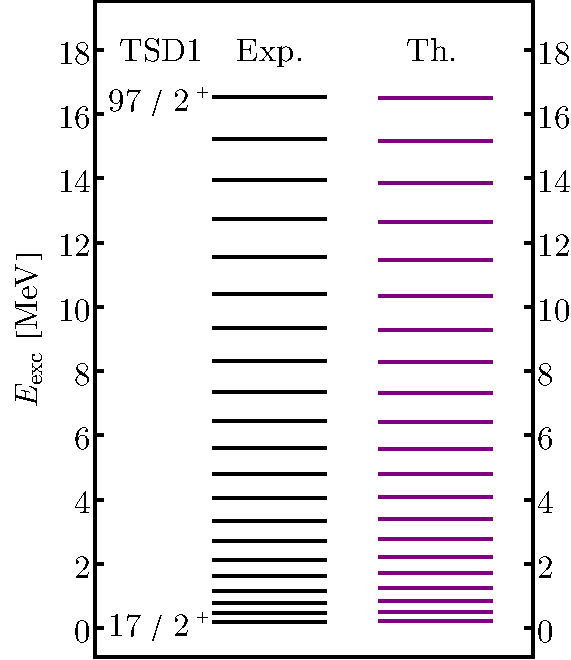
\includegraphics[width=0.49\textwidth]{Chapters/Figures/parity-partners-plots/tsd1.pdf}
    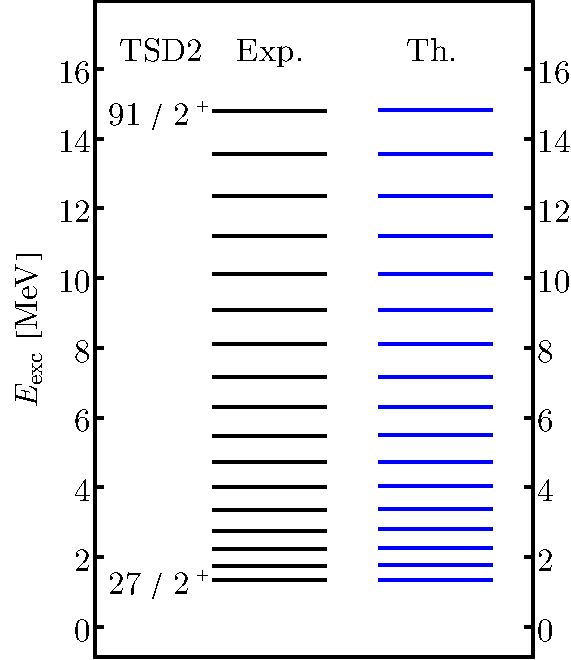
\includegraphics[width=0.49\textwidth]{Chapters/Figures/parity-partners-plots/tsd2.pdf}
    \caption{The excitation energies (Eq. \ref{general-excitation-energy-fitting-model}) of $^{163}$Lu for the bands TSD1 and TSD2, obtained in the $\mathbf{W_2}$ formalism using Eq. \ref{tsd-energies-lu163-parity-partners}. Calculations were done with the parameters presented in Table \ref{lu163-parameters-parity-fitting}.}
    \label{results-parity-partners-163lu-1}
\end{figure}
\begin{figure}
    \centering
    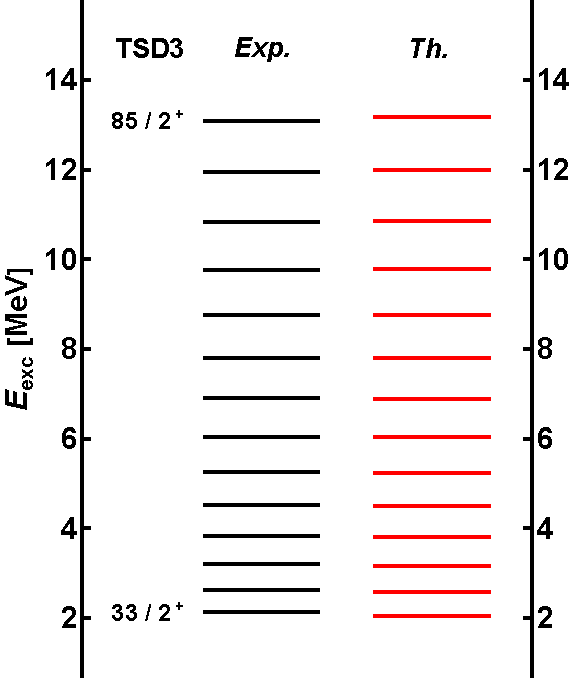
\includegraphics[width=0.49\textwidth]{Chapters/Figures/parity-partners-plots/tsd3.pdf}
    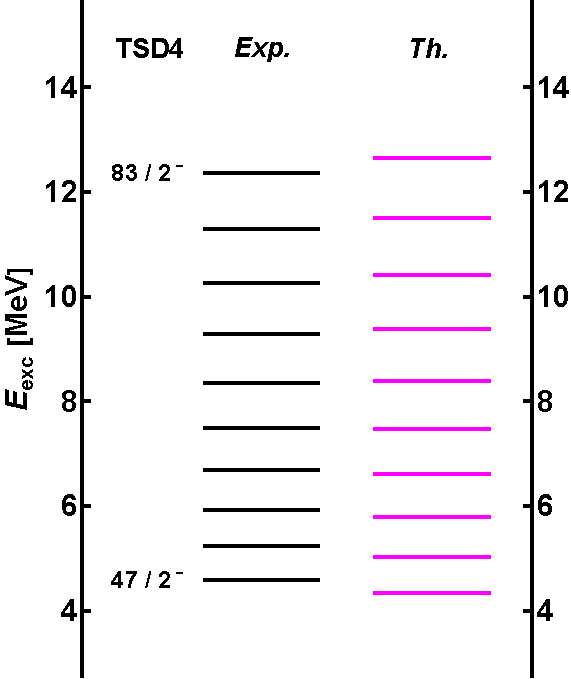
\includegraphics[width=0.49\textwidth]{Chapters/Figures/parity-partners-plots/tsd4.pdf}
    \caption{The excitation energies (Eq. \ref{general-excitation-energy-fitting-model}) of $^{163}$Lu for the bands TSD3 and TSD4 , obtained in the $\mathbf{W_2}$ formalism using Eq. \ref{tsd-energies-lu163-parity-partners}. Calculations were done with the parameters presented in Table \ref{lu163-parameters-parity-fitting}.}
    \label{results-parity-partners-163lu-2}
\end{figure}

Also worth discussing is the difference $\delta_{42}=E_I^\text{TSD4}-E_I^\text{TSD2}$, where the almost constant value $\delta_{42}\approx 0.3\ \text{MeV}$ is observed, suggesting that the states with the same angular momentum from TSD2 and TSD4 might emerge from the parity projection of a single wave-function lacking reflection symmetry (hence the change $\pi=+1\to\pi=-1$). For the sake of completeness, the two wobbling frequencies $\Omega_{1,2}$ that comprise the phonon term $\mathcal{F}^I_{n_{w_1}n_{w_2}}$ defined in Eq. \ref{phononic-term-tsd-energies} are also represented as function of the total angular momentum in Fig. \ref{lu163-wobbling-frequencies-parity}. It can be seen that the solution $\Omega_2$ is much larger over the entire spin range, indicating that the odd proton's a.m. exhibits a more pronounced precessional motion than that of the core. Indeed, the difference is only about $1.5-2\ \text{MeV}$ for low $I$ and it goes to $3.5-4\ \text{MeV}$ in the large spin limit. Nevertheless, this is expected because the condition $\Omega_2>\Omega_1$ was fixed in Eq. \ref{omega-1-2-3-4-solutions}.
\begin{figure}
    \centering
    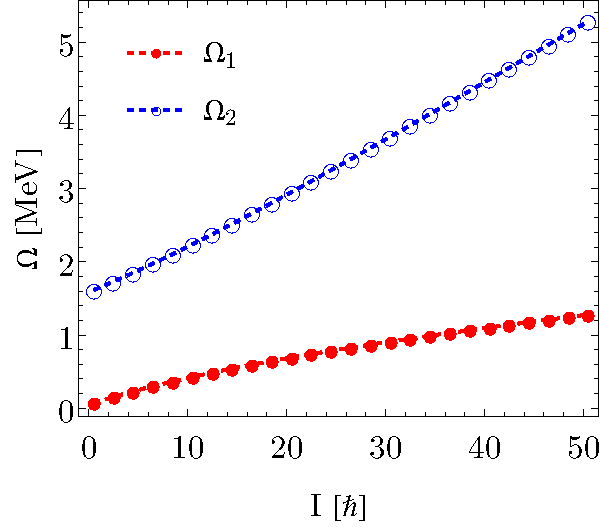
\includegraphics[scale=0.8]{Chapters/Figures/parity-partners-plots/wobblingFrequency.pdf}
    \caption{The wobbling frequencies, i.e., the two solutions of Eq. \ref{wobbling-freq-oddA} as function of the total spin. Calculations are made with the parameter set provided in Table \ref{lu163-parameters-parity-fitting}.}
    \label{lu163-wobbling-frequencies-parity}
\end{figure}

\subsection{Parameter set - Interpretation}

The set $\mathcal{P}_\text{fit}$ attained after the minimization procedure of the $\chi^2$-function is given in Table \ref{lu163-parameters-parity-fitting}. However, the fitting method only gives the numerical values, without providing context on the physical interpretation of the results themselves. As such, in this subsection one should make a quantitative analysis for the five parameters and see how the current model compares with existing studies. Concerning the magnitudes of the three moments of inertia, it is clear that the system rotates around the $1$-axis, as the largest MOI corresponds to this axis. Moreover, the $1$-axis MOI is much larger than the other two, signifying the nature of small-amplitude vibrations that are typical to a triaxial rotor (i.e., large rotational motion around $\mathcal{I}_1$ and a fluctuation generated by the anisotropy of $\mathcal{I}_{2,3}$). A graphical representation where the three moments of inertia are compared with the $\mathbf{W_1}$ formalism is shown in Fig. \ref{moi-comparison-w1-w2-formalisms}. Looking at the plot, it can be seen that $\mathcal{I}_1$ is the largest across all the fitting procedures, although $\mathbf{W_2}$ provides the largest one. It should be pointed out that these are \emph{effective} MOI of the system, that is the particle + triaxial-rotor. There is no spin dependence inferred for the three quantities, so a possible change in their ordering cannot be studied with the current description. Since the current approach is not a microscopic one, no presumptions on that causes the MOI ordering can be stated (e.g., orbital mixing and so on). As a matter of fact, the nature of the three MOI for a real nucleus is neither rigid nor irrotational (see discussion from Chapter \ref{chapter-3} and Eq. \ref{experimental-MOI-vs-rig-irr}).
\begin{figure}
    \centering
    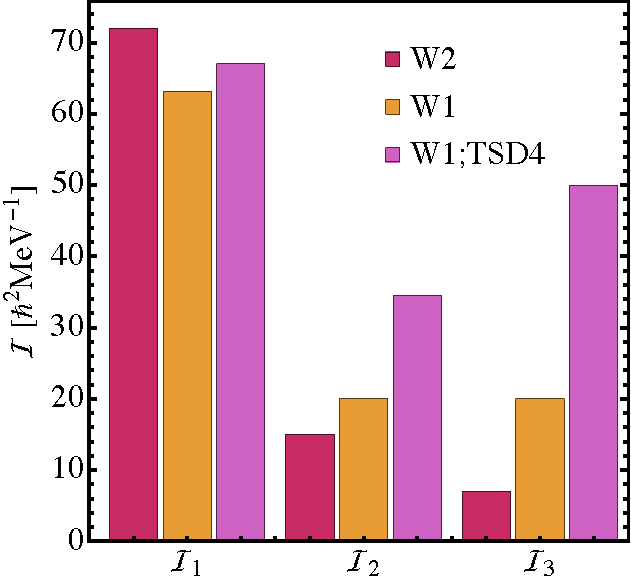
\includegraphics[scale=0.75]{Chapters/Figures/parity-partners-plots/W1-W2-Mois.pdf}
    \caption{Comparison between the MOI obtained in the approach $\mathbf{W_2}$ (current chapter) and $\mathbf{W_1}$ (as per Chapter \ref{chapter-6-aw1-formalism}). Note that there was a separate minimization of the $\chi^2$-function for TSD4 within the previous formalism. The numerical values for $\mathcal{I}_{1,2,3}$ are taken from Tables \ref{numerical-fitting-parameters-Lu-isotopes} and \ref{lu163-parameters-parity-fitting}.}
    \label{moi-comparison-w1-w2-formalisms}
\end{figure}

Taking the moments of inertia given by the $\mathbf{W_2}$ model, a direct comparison with the rigid and hydrodynamical (irrotational) ones is made in Fig. \ref{w2-mois-comparison}. The rigid values are calculated using the first formula from Eq. \ref{eq-irrotational-rigid-mois} and the hydrodynamical values are attained using the second formula. It is noteworthy that the MOI provided by the fit suggest an irrotational-like behavior rather than a rigid-like for the triaxial system, since there is a larger discrepancy between the MOI of the $2$- and $3$-axes in the rigid case.
\begin{figure}
    \centering
    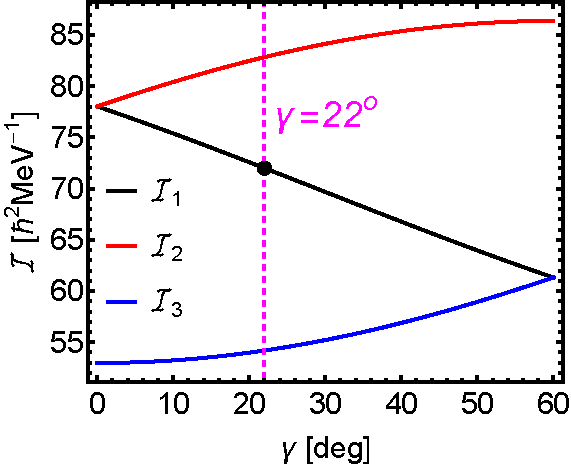
\includegraphics[width=0.49\textwidth]{Chapters/Figures/parity-partners-plots/rigid-mois-fit.pdf}
    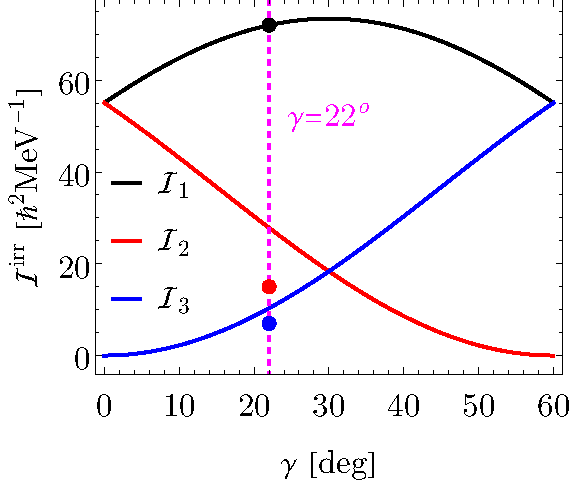
\includegraphics[width=0.49\textwidth]{Chapters/Figures/parity-partners-plots/hydrodynamic-mois-fit.pdf}
    \caption{The rigid (\textbf{left}) and hydrodynamical (\textbf{right}) MOI as function of $\gamma$. The scaling factors for both types of MOI are determined by fixing $\mathcal{I}^\text{rig}_1$ and $\mathcal{I}_1^\text{irr}$ to the fitted $\mathcal{I}_1$ with the deformation parameters $(\beta,\gamma)=(0.38,22^\circ)$. The black, red, and blue points represented the numerical values of $\mathcal{I}_1$, $\mathcal{I}_2$, and $\mathcal{I}_3$ from Table \ref{lu163-parameters-parity-fitting}, respectively. The value $\gamma=22^\circ$ from the fit is marked with the dashed magenta line just to guide the eye.}
    \label{w2-mois-comparison}
\end{figure}

Going further with the analysis of the parameters, a value of $\gamma=22^\circ$ is obtained. The agreement with the predicted minimum of $^{163}$Lu \cite{jensen2002wobbling,jensen2004coexisting} is quite good, as the experimental minimum for the TSD structures is identified at $(\beta,\gamma)=(0.38,20^\circ)$ (recall Fig. \ref{pes-example-set-2}). Other studies that describe the wobbling properties of $^{163}$Lu take the triaxiality parameter fixed a priori (see Refs. \cite{tanabe2006algebraic,tanabe2017stability} for example), but the current approach determines $\gamma$ self-consistently. Remarkable the fact that the obtained value is slightly bigger than the one from $\mathbf{W_1}$ ($\gamma=17^\circ$). This might be caused by the larger ratios for $\mathcal{I}_1/\mathcal{I}_2=4.8$ and $\mathcal{I}_1/\mathcal{I}_3=10.2$ in $\mathbf{W_2}$ than the ones from $\mathbf{W_1}$ ($\mathcal{I}_1/\mathcal{I}_2=3.1$ and $\mathcal{I}_1/\mathcal{I}_3=6.3$, respectively), which also indicate a larger triaxiality.

Lastly, the single-particle potential strength should be discussed. It has a value of $V=2.1\ \text{MeV}$ and in $\mathbf{W_1}$ this parameter was $V^{\text{TSD1,2,3}}=3.1\ \text{MeV}$ and $V^\text{TSD4}=0.7\ \text{MeV}$. An explanation for its decrease in the present case might be due to the upward shift in the energy caused by the unfavored partner, or due to the energetic shift of the parity partner. Nevertheless, a quenching effect on the quadrupole deformation of the triaxial system due to either the signature splitting or the parity symmetry breaking is observed. Still, the obtained value seems to be consistent with the previous calculations, as $V$ is close to the average value of the two $V$'s from $\mathbf{W_1}$. Other interpretations developed using a similar single-particle term in the Hamiltonian adopted values around $V=1.6\ \text{MeV}$ \cite{tanabe2017stability}, however, that was for an isotope with smaller quadrupole deformation $\beta_2=0.18$.

According to the structure described in the beginning of this chapter, the above sections conclude part $1)$ of the research, which was supposed to describe the concept of Parity Partners, to re-define the excitation energy spectrum and apply it to $^{163}$Lu, and finally to give a some context on the interpretation of the free parameters. Since all points were properly covered, and one can go further to part $2)$ of this study, where the classical energy function must be re-evaluated under the assumptions of $\mathbf{W_2}$ approach.

\section{Classical Energy Function (CEF)}

From the Hamiltonian given by Eq. \ref{total-ham-approach-w1} (i.e., sum of the single-particle term in Eq. \ref{single-particle-ham-approach-w1} and the rotor term in Eq. \ref{rotor-ham-approach-w1}), one obtained the classical energy function by taking the Hamiltonian's average on the trial function (Eq. \ref{trial-function-appeoach-w1}). The structure of the CEF was firstly given in Section \ref{classical-energy-function-subsection} and even a qualitative analysis of its sub-terms has been employed in Figs. \ref{fig-A-varphi-canonical} - \ref{fig-A-gamma-canonical}. The minimum point of $\mathcal{H}$ was found to be $p_0=(0,I;0,j)$ (recall Eq. \ref{cef-minimum-point-p0}). These considerations are still important here. Adopting the polar coordinate system $(\theta,\varphi)$, the Cartesian components of the total angular momentum can be expressed as:
\begin{align}
    \mathbf{I}=&\left\{I_1,I_2,I_3\right\}\stackrel{not.}{=}\left\{x_1,x_2,x_3\right\}\ ,\nonumber\\
    x_1=I\sin\theta\cos\varphi\ ,&\ x_2=I\sin\theta\sin\varphi\ ,\ x_3=I\cos\theta\ ,
    \label{polar-coordinates-total-AM}
\end{align}
where the quantization axis is chosen as the $3$-axis. Going back to the expression of $\mathcal{H}$ from Eq. \ref{full-classical-energy-function} and evaluating it in the minimum point using the new coordinate system, a compact form is achieved \cite{poenaru2021extensive2}:
\begin{align}
    \left. \mathcal{H}\ \right\vert_{p_0}=I\left(I-\frac{1}{2}\right)\sin^2\theta\cdot \mathcal{A}_\varphi-2A_1Ij\sin\theta+T_\text{core}+T_\text{sp}\ ,
    \label{CEF-minimum-point-Tcore-Tsp}
\end{align}
where the last two terms are independent of the polar angles $(\theta,\varphi)$ and they are defined as \cite{poenaru2021extensive2}:
\begin{align}
    T_\text{core}&=\frac{I}{2}(A_1+A_2)+A_3I^2\ ,\\
    T_\text{s.p.}&=\frac{j}{2}(A_2+A_3)+A_1j^2-V\frac{2j-1}{j+1}\sin\left(\gamma+\frac{\pi}{6}\right)\ .
    \label{core-sp-sub-terms}
\end{align}

It would be instructive to see how the core factor from Eq. \ref{core-sp-sub-terms} behaves under different $A_k$ orderings and also how the single-particle term evolves for different $j$. Two such comparisons are depicted in Fig \ref{fig-t-core-sp-terms}. The variations of $T_\text{sp}$ at different $j$ values are not significant. On the other hand, the $A_k$ ordering affects $T_\text{core}$ with a large amount, especially for higher spins.
\begin{figure}
    \centering
    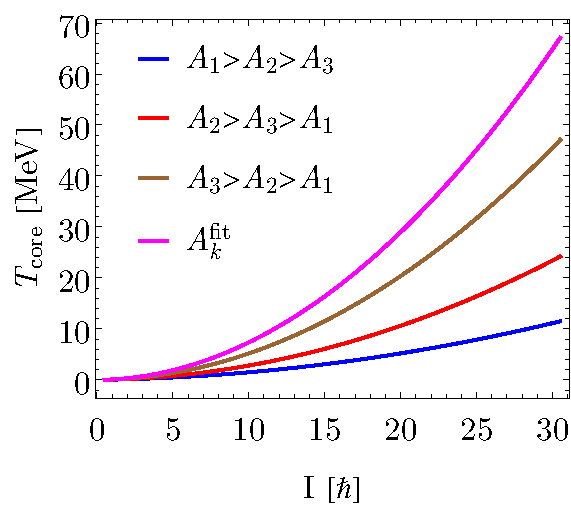
\includegraphics[width=0.48\textwidth]{Chapters/Figures/parity-partners-plots/t-core.pdf}
    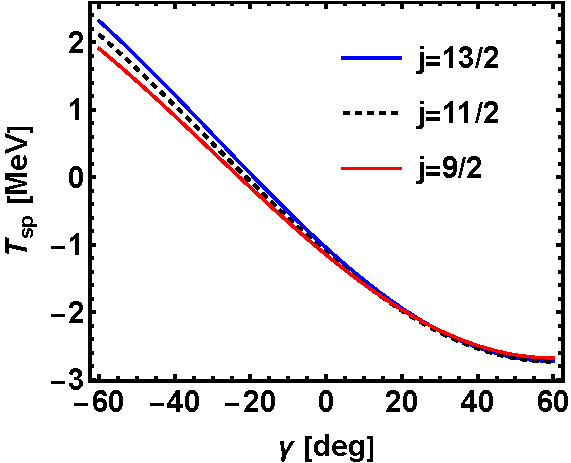
\includegraphics[width=0.495\textwidth]{Chapters/Figures/parity-partners-plots/t-sp.pdf}
    \caption{\textbf{Right:} The term $T_\text{core}$ from Eq. \ref{core-sp-sub-terms} as function of the angular momentum $I$ at different orderings for $A_k$ (the arbitrary values $0.05, 0.025, 0.011\ \hbar^{-2}\text{MeV}$ were interchanged between each factor). The magenta line is for the inertia factors provided by the fit. \textbf{Left:} The term $T_\text{sp}$ from Eq. \ref{core-sp-sub-terms}, evaluated for three different single-particle angular momenta using the potential strength and the three MOI from Table \ref{lu163-parameters-parity-fitting}.}
    \label{fig-t-core-sp-terms}
\end{figure}

\subsection{CEF - Stability Regions}

The classical energy function from Eq. \ref{CEF-minimum-point-Tcore-Tsp} is expressed as using the classical coordinates that describe the dynamics of the core (i.e., $r,\varphi$) and the valence nucleon (i.e., $f,\psi$). However, $\mathcal{H}(r,\varphi;f,\psi)$ is nothing else than the average of $\hat{H}$ on the trial function. Going back into the quantal picture, the physical interpretation of Eq. \ref{CEF-minimum-point-Tcore-Tsp} is thus: \emph{the expectation value of the Hamiltonian} or \emph{the allowed energy states that the total system can have}. For this reason, analyzing the CEF around the critical points is crucial for identifying stability of the system concerning its the rotational motion. In this subsection, such calculations will be performed, namely the critical points of $\mathcal{H}$ will be identified and then graphical representations in the polar plane $(\theta,\varphi)$ will be made. If there are extremal points with minimum character present, then the so-called regions of stability could be pinpointed. These regions should indicate if there are any allowed rotational states for the system.

Firstly, all the critical points with minimum character for $\mathcal{H}$ are given in Table \ref{critical_points_h}. Furthermore, by fixing the intervals of variation for $\theta$ and $\varphi$ to be $\theta\in[0,\pi]$ and $\varphi\in[0,2\pi]$, respectively, some numerical evaluations for the CEF can be realized in this coordinate space. These are finally sketched as \emph{contour plots} for different spins belonging to the four triaxial bands in $^{163}$Lu. For the sake of completeness, contour plots for two spin states from each band will be constructed, and moreover, the critical points from Table \ref{critical_points_h} are drawn in these figures. The plots are shown in Figs. \ref{contour-cef-polar-tsd1} - \ref{contour-cef-polar-tsd4}.
\begin{table}
    \centering
    \begin{tabular}{cccc}
    \hline
    Minimal point & $\theta$ [rad] & $\varphi$ [rad] & $A_k$ ordering \\
    \hline
    \hline
    $m_1$ & $\pi/2$ &   $0$     &   $A_3>A_2>A_1$   \\
    $m_2$ & $\pi/2$ &   $\pi$   &   $A_3>A_2>A_1$   \\
    $m_3$ & $\pi/2$ &   $2\pi$  &   $A_3>A_2>A_1$   \\
    \hline
    \end{tabular}
    \caption{The minimum points of $\mathcal{H}$ for a fixed ordering of the inertia factors. The ordering of $A_k$ is chosen in agreement with the fit parameters from Table \ref{lu163-parameters-parity-fitting}.}
    \label{critical_points_h}
\end{table}
\begin{figure}
    \centering
    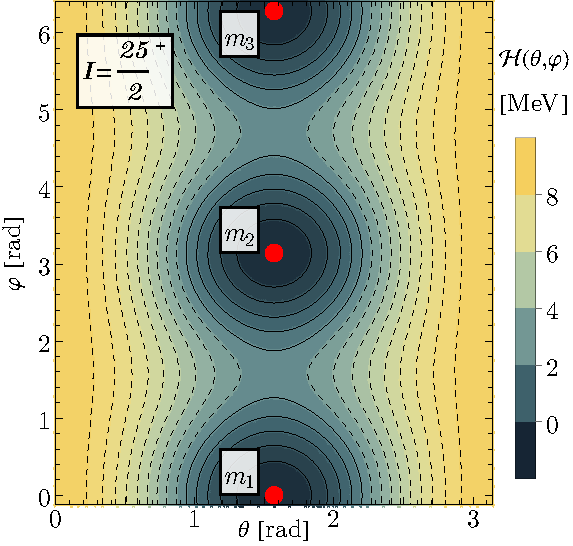
\includegraphics[width=0.49\textwidth]{Chapters/Figures/parity-partners-plots/contour-tsd1-1.pdf}
    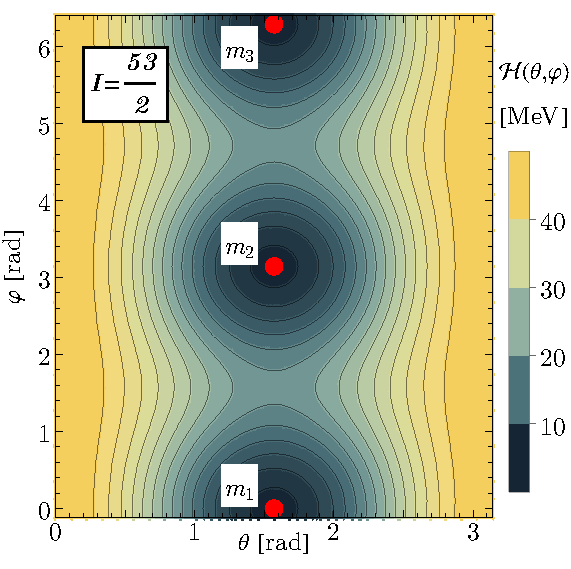
\includegraphics[width=0.49\textwidth]{Chapters/Figures/parity-partners-plots/contour-tsd1-2.pdf}
    \caption{The classical energy function (Eq. \ref{CEF-minimum-point-Tcore-Tsp}) expressed in terms of the polar coordinates for two states from TSD1 (i.e., $I=25/2^+$ and $53/2^+$). The calculations are done using the fit parameters (see Table \ref{lu163-parameters-parity-fitting}). Darker color signifies lower values. The minimum points of $\mathcal{H}$ are marked by the red dots and are surrounded by closed contours. See text for explanation on the dashed contour styling.}
    \label{contour-cef-polar-tsd1}
\end{figure}
\begin{figure}
    \centering
    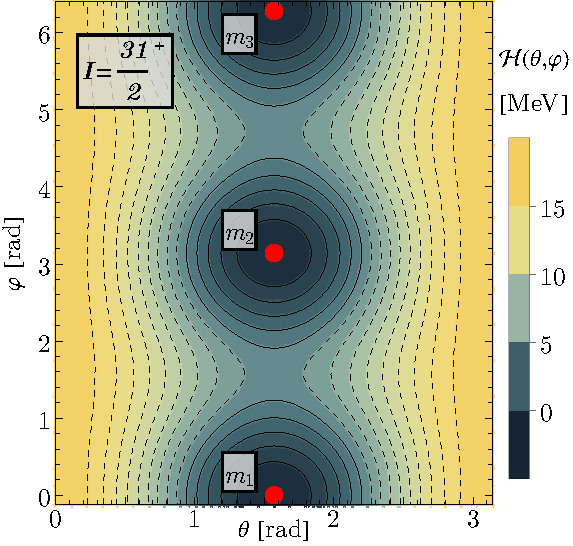
\includegraphics[width=0.49\textwidth]{Chapters/Figures/parity-partners-plots/contour-tsd2-1.pdf}
    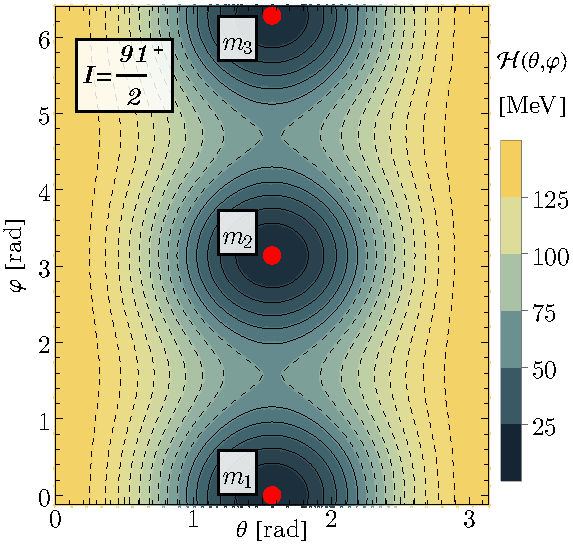
\includegraphics[width=0.49\textwidth]{Chapters/Figures/parity-partners-plots/contour-tsd2-2.pdf}
    \caption{The classical energy function (Eq. \ref{CEF-minimum-point-Tcore-Tsp}) expressed in terms of the polar coordinates for two states from TSD2 (i.e., $I=31/2^+$ and $91/2^+$). The calculations are done using the fit parameters (see Table \ref{lu163-parameters-parity-fitting}). Darker color signifies lower values. The minimum points of $\mathcal{H}$ are marked by the red dots and are surrounded by closed contours. See text for explanation on the dashed contour styling.}
    \label{contour-cef-polar-tsd2}
\end{figure}
\begin{figure}
    \centering
    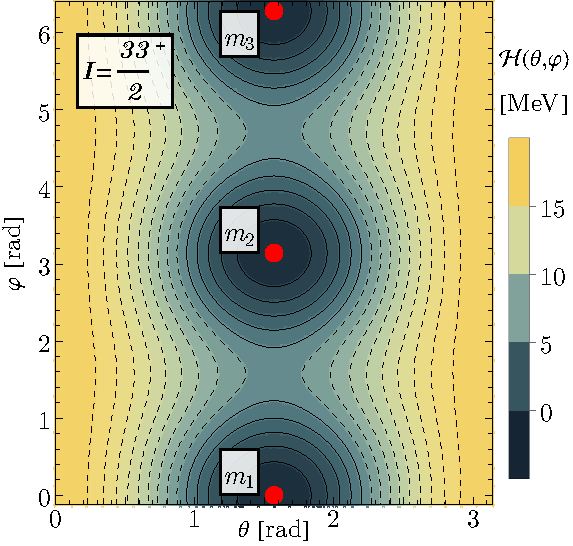
\includegraphics[width=0.49\textwidth]{Chapters/Figures/parity-partners-plots/contour-tsd3-1.pdf}
    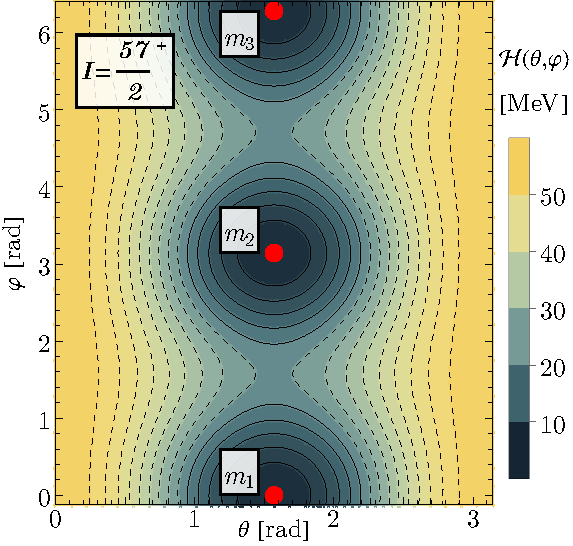
\includegraphics[width=0.49\textwidth]{Chapters/Figures/parity-partners-plots/contour-tsd3-2.pdf}
    \caption{The classical energy function (Eq. \ref{CEF-minimum-point-Tcore-Tsp}) expressed in terms of the polar coordinates for two states from TSD3 (i.e., $I=33/2^+$ and $57/2^+$). The calculations are done using the fit parameters (see Table \ref{lu163-parameters-parity-fitting}). Darker color signifies lower values. The minimum points of $\mathcal{H}$ are marked by the red dots and are surrounded by closed contours. See text for explanation on the dashed contour styling.}
    \label{contour-cef-polar-tsd3}
\end{figure}
\begin{figure}
    \centering
    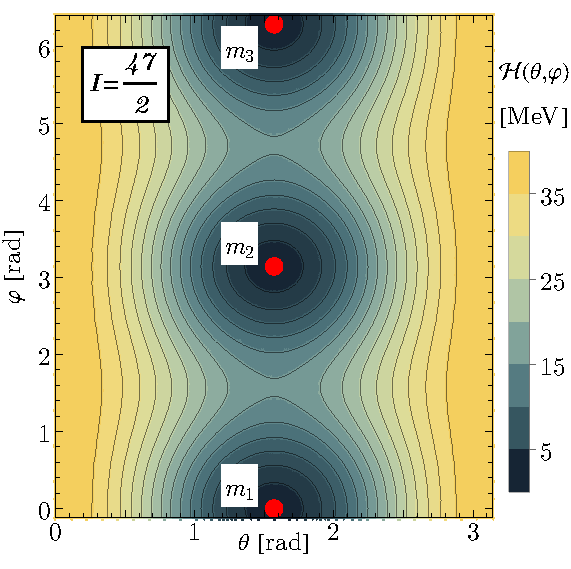
\includegraphics[width=0.49\textwidth]{Chapters/Figures/parity-partners-plots/contour-tsd4-1.pdf}
    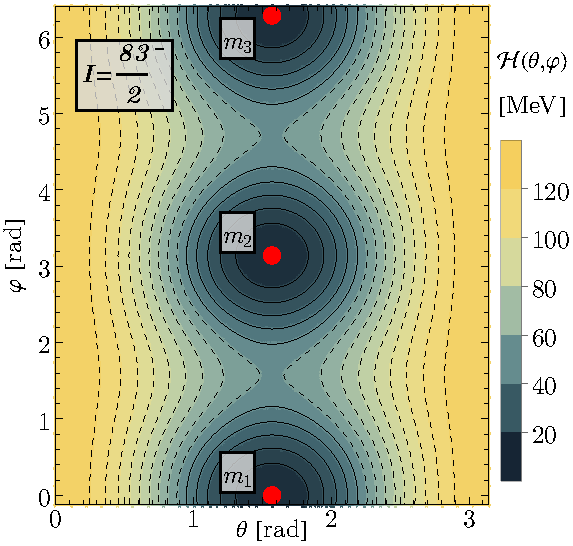
\includegraphics[width=0.49\textwidth]{Chapters/Figures/parity-partners-plots/contour-tsd4-2.pdf}
    \caption{The classical energy function (Eq. \ref{CEF-minimum-point-Tcore-Tsp}) expressed in terms of the polar coordinates for two states from TSD4 (i.e., $I=47/2^-$ and $83/2^-$). The calculations are done using the fit parameters (see Table \ref{lu163-parameters-parity-fitting}). Darker color signifies lower values. The minimum points of $\mathcal{H}$ are marked by the red dots and are surrounded by closed contours. See text for explanation on the dashed contour styling.}
    \label{contour-cef-polar-tsd4}
\end{figure}

Looking at the set of graphics depicted in Figs. \ref{contour-cef-polar-tsd1} - \ref{contour-cef-polar-tsd4}, some remarking features emerge. They have some similarities, suggesting resembling collective properties, but also some discrepancies, caused by the different depths of the minima. A primary common feature consists of the set of equi-energy curves that surround a sole minimum point for the low values of $\mathcal{H}(\theta,\varphi)$. Around the minimum point $m_2$ there are closed trajectories (marked by the solid black lines) and as the energy increases (keeping the angular momentum fixed) there is a \emph{critical region} at which the orbits surround all minima (highlighted by the dashed lines). The lack of localization for these orbits indicate an \emph{unstable motion} of the nucleus and they could be related to a phase transition, where the system undergoes a sudden change in its rotational character. Indeed, examining Fig. \ref{contour-cef-polar-tsd2}, which has quite deep minima (as the maximal values reach $\approx 120\ \text{MeV}$), there are about five stable trajectories that surround $m_{1,2,3}$. Beyond those trajectories, the wobbling motion becomes unstable. From an equilibrium standpoint, such `excited' states cannot be reached by the nucleus, hence the rotational motion occurs near the minimum points. Discussion on the stability of the wobbling motion will be reiterated in the next section, but it is worth mentioning that such a description for the dynamics of a nucleus in terms of classical orbits is a unique feature of this research.

Additionally, the CEF is studied quantitatively in one of its minimum points (i.e., the $m_1=(\pi/2,0)$ point from Table \ref{critical_points_h}) w.r.t. the total angular momentum. As the depth of the contour plots changes across the different spin states, it would be instructive to see how these modifications are affected by $I$. As a result, a graphical representation of $\mathcal{H}$ in the point $m_2$ has been sketched in Fig. \ref{CEF-m2-I-dependence}. As a final step in this analysis, Fig. \ref{CEF-theta-phi-dependence} shows the behavior of $\mathcal{H}$ with respect to different values of $I$, by keeping one polar coordinate fixed and varying the other. The fixed values are taken to coincide with the minimum point $m_1$.
\begin{figure}
    \centering
    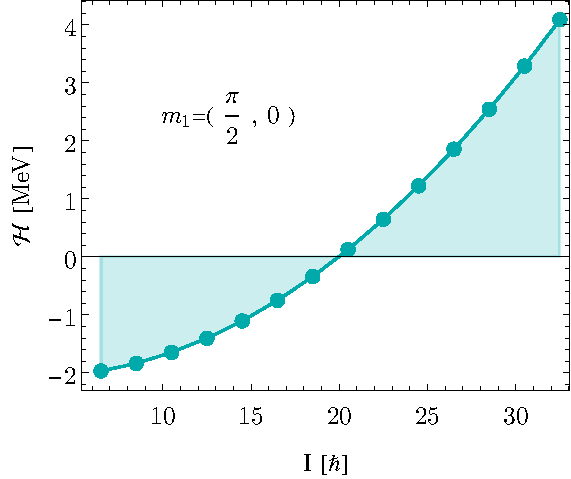
\includegraphics[scale=0.75]{Chapters/Figures/parity-partners-plots/H-minimal-m1.pdf}
    \caption{The CEF from Eq. \ref{CEF-minimum-point-Tcore-Tsp} is evaluated in one of its minimum points ($m_1=(\pi/2,0)$ given in Table \ref{critical_points_h}) and plotted with respect to the angular momentum. The calculations are done using the fitting parameters from Table \ref{lu163-parameters-parity-fitting}.}
    \label{CEF-m2-I-dependence}
\end{figure}
\begin{figure}
    \centering
    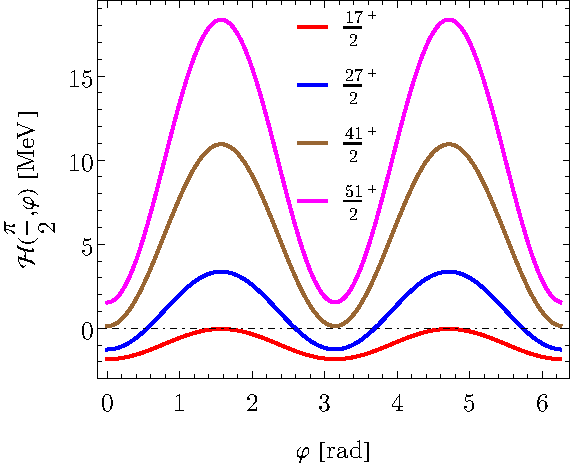
\includegraphics[width=0.5\textwidth]{Chapters/Figures/parity-partners-plots/H-minimal-m1-phi.pdf}
    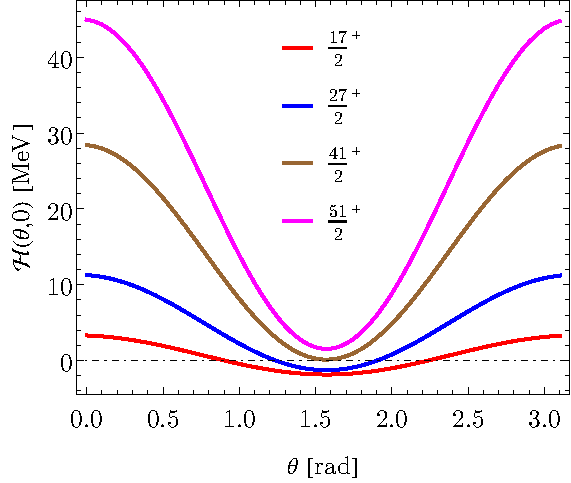
\includegraphics[width=0.485\textwidth]{Chapters/Figures/parity-partners-plots/H-minimal-m1-theta.pdf}
    \caption{The evolution of $\mathcal{H}$ for different values of $I$, obtained by keeping one polar coordinate fixed and letting the other one vary in its normal interval. \textbf{Left:} The coordinate $\theta$ is fixed to $\theta=\pi/2$ and $\varphi=[0,2\pi]$. \textbf{Right:} The coordinate $\varphi$ is fixed to $\varphi=0$ and $\theta=[0,\pi]$.}
    \label{CEF-theta-phi-dependence}
\end{figure}

By expressing the classical energy function in terms of the polar coordinates, an analytical structure of Eq. \ref{CEF-minimum-point-Tcore-Tsp} is properly obtained. This function provides an insight into the precessional motion of the angular momentum, which according to the calculations made for $^{163}$Lu in the $\mathbf{W_2}$ approach, is the $1$-axis (largest MOI is $\mathcal{I}_1$). The representations shown in Figs. \ref{contour-cef-polar-tsd1} - \ref{contour-cef-polar-tsd4} depict three regions, i.e., i) one where the triaxial ellipsoid could behave as a wobbler, having closed circular orbits around $m_{1,2,3}$ ii) a criticality region and iii) $\mathcal{H}>\mathcal{H}_\text{critical}$ beyond which the orbits become non-localized and surround all three minima. This critical value can be extracted from the left inset of Fig \ref{CEF-theta-phi-dependence} as the peak value. A simple sketch where all these regions can be clearly differentiated is made in Fig. \ref{fig-H-unstable-sketch}. Identification of a phase transition between a well-defined motion around $1$-axis and an unstable rotor is a remarking feature in the current model.
\begin{figure}
    \centering
    \includegraphics[scale=1]{Chapters/Figures/parity-partners-plots/H-unstable-edited.pdf}
    \caption{A schematic illustration showing the three regions that can be identified for a triaxial nucleus within the $\mathbf{W_2}$ formalism. The stable motion is characterized by the closed orbits around the minimal points $m_{1,2,3}$ suggesting the precession of $\mathbf{I}$ around the $1$-axis. Furthermore, for a fixed angular momentum, a critical value of $\mathcal{H}$ is marked by the thick orange lines. Beyond this region, the rotational motion becomes unstable, signaling a phase transition.}
    \label{fig-H-unstable-sketch}
\end{figure}

\subsection{Classical 3D Trajectories}

In the previous section, a study of the wobbling motion in $^{163}$Lu has been performed in terms of the classical energy function. However, the analysis was only elaborated in the space generated by the set of polar coordinates (Eq. \ref{polar-coordinates-total-AM}), restricting the geometrical interpretation of the system dynamics to a two-dimensional picture. In two recent publications \cite{poenaru2021extensive1,poenaru2021extensive2}, the team successfully gave a $3$-dimensional representation of the classical energy function. In the following, the numerical recipe for obtaining this geometry will be presented.

From the classical equations of motion depicted in Chapter \ref{chapter-6-aw1-formalism}, it results that the system admits two constants of motion, i.e., the total energy and the total angular momentum. These two quantities are obviously expected to be conserved. The angular momentum can be written as the squared sum of its components:
\begin{align}
    I^2=x_1^2+x_2^2+x_3^2\ .
    \label{constant-of-motion-I}
\end{align}

Using the initial CEF provided in Eq. \ref{CEF-minimum-point-Tcore-Tsp}, one can aim at expressing it in terms of $x_1$, $x_2$, and $x_3$, respectively. This would imply that the energy function explicitly contains the angular momentum components. Changing from the polar coordinates to the cartesian ones $\mathcal{H}(\theta,\varphi)\longrightarrow E(x_1,x_2,x_3)$, the following formula for the energy is obtained \cite{poenaru2021extensive2}:
\begin{align}
    E=&\left(1-\frac{1}{2I}\right)A_1x_1^2+\left(1-\frac{1}{2I}\right)A_2x_2^2+\left[\left(1-\frac{1}{2I}\right)A_3+A_1\frac{j}{I}\right]x_3^2\nonumber\\
    &-I\left(I-\frac{1}{2}\right)A_3-2A_1Ij+T_\text{rot}+T_\text{sp}\ .
    \label{constant-of-motion-E}
\end{align}
where $E$ is now called the \emph{energy surface} \cite{poenaru2021extensive2}. In the expression of $E$, one can notice the three coordinates $x_k$ that appear as squared terms. If some notations are introduced and some algebraic manipulations are performed, the energy surface acquires the compact form:
\begin{align}
    E'=\frac{x_1^2}{s_1}+\frac{x_2^2}{s_2}+\frac{x_3^2}{s_3}\ ,
    \label{energy-surface-E}
\end{align}
where $E'$ is the energy after the $x_k$-free terms in the r.h.s. of Eq. \ref{constant-of-motion-E} have been subtracted from $E$. The structure of Eq. \ref{energy-surface-E} resembles a general ellipsoid (hence the name \emph{energy surface}):
\begin{align}
    \frac{x_1^2}{a^2}+\frac{x_2^2}{b^2}+\frac{x_3^2}{c^2}=1\ ,
\end{align}
where $a,b,c$ are the semi-axes of different length, which for the triaxial ellipsoid become:
\begin{align}
    a\to\sqrt{E's_1}\nonumber\ ,\\
    b\to\sqrt{E's_2}\nonumber\ ,\\
    c\to\sqrt{E's_3}\ .
    \label{semi-axes-lenghts-E}
\end{align}

The semi-axes lengths depend on the three inertia factors $A_k$, meaning that the fit quality will be also reflected into the geometrical shape of $E'$ through the parameter set $\mathcal{P}_\text{fit}$. Putting together Eq. \ref{constant-of-motion-I} (i.e., a sphere of radius $r=I$) and Eq. \ref{energy-surface-E} (an ellipsoid with semi-axes given by Eq. \ref{semi-axes-lenghts-E}), their intersection can be made in the 3-dimensional space generated by the angular momentum components $\left\{x_1,x_2,x_3\right\}$. These overlapping surfaces will give the \emph{classical trajectories}, defined as a collection of points in this space along which the total angular momentum $\mathbf{I}$ is orbiting, making a precessional motion. These trajectories will play a crucial role in characterizing the motion of the nucleus, as they will be oriented along one of the three axes $x_k\ ,\ k=1,2,3$, suggesting rotations around a particular direction preferred by the system.

When the model PRM Hamiltonian (Eq. \ref{total-ham-approach-w1}) is diagonalized for a given $I$, a set of $2I+1$ energies are obtained. Thus, it is mandatory to study the evolution of these trajectories when the nucleus' energy increases and see their behavior with respect to the angular momentum and energy. The intersection curves of the two constants of motion Eq. \ref{constant-of-motion-I} and Eq. \ref{constant-of-motion-E} are represented as manifolds in Figs. \ref{classical-trajectory-TSD1-plot} - \ref{classical-trajectory-TSD4-plot}, where each figure represents a rotational state within one of the four bands of $^{163}$Lu. Every representation contains three insets that reveal different nuclear phases. The first inset (left) shows the trajectory of the system given by the intersection between the angular momentum $I$ and the real energy of this state (according to the experimental data from Figs. \ref{results-parity-partners-163lu-1} - \ref{results-parity-partners-163lu-2}). Therefore, it can be regarded as the `real' nuclear trajectory, and it is remarkable the fact that all the real trajectories are observed along the $x_1$-axis. The invariance of $\hat{H}$ to rotations with $\pi$ about $x_1$ makes it possible to have two distinct (although symmetrical) paths along $x_1$, i.e., one around the positive direction and one around the negative direction, which are clearly depicted with red ellipses encompassing this axis. Keep in mind that the energy surface is evaluated using the parameters $\mathcal{P}_\text{fit}$, therefore one expects $x_1$ to be the rotational axis.
\begin{figure}
    \centering
    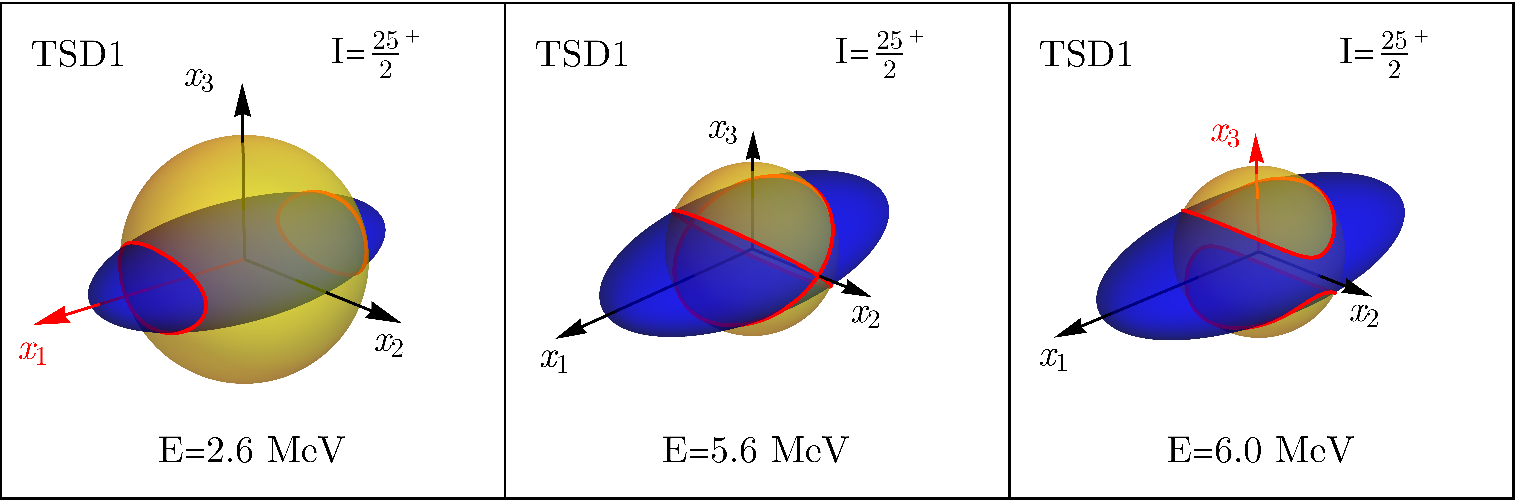
\includegraphics[width=0.99\textwidth]{Chapters/Figures/parity-partners-plots/classical-trajectory-TSD1.pdf}
    \caption{The nuclear trajectories for the state $I=25/2^+$ from TSD1 in $^{163}$Lu. The left inset shows the trajectory of the system corresponding to the real energy of this particular spin (i.e., the red ellipses that surround $x_1$). The rotational axis is marked by the red color, signifying that the nucleus wobbles around it. See text for more details.}
    \label{classical-trajectory-TSD1-plot}
\end{figure}
\begin{figure}
    \centering
    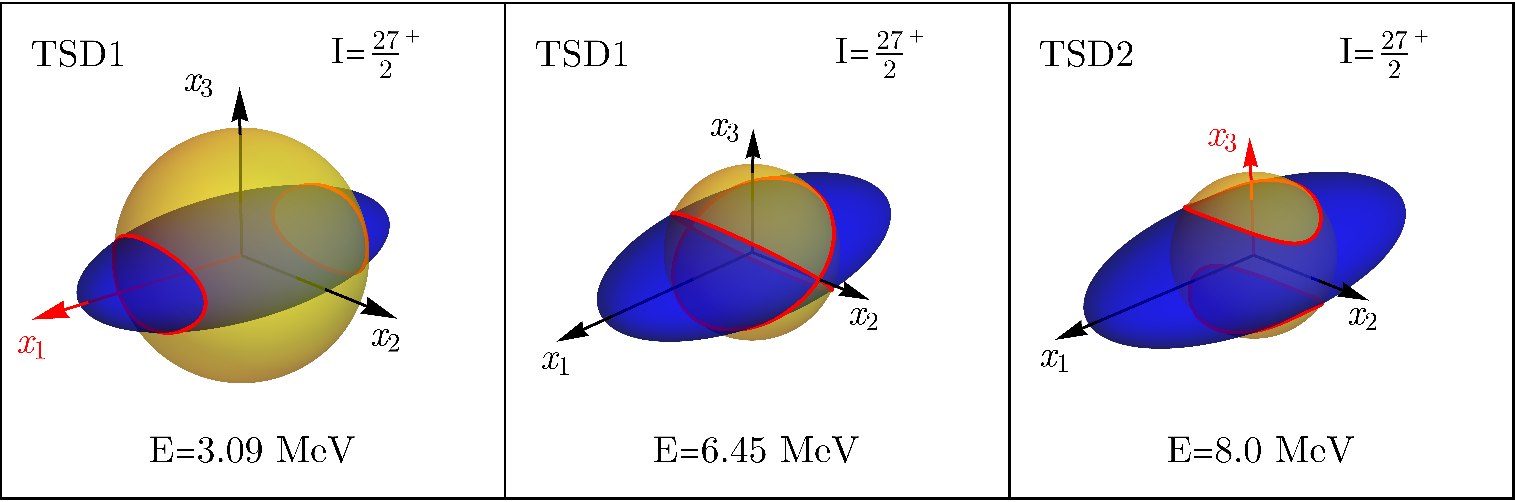
\includegraphics[width=0.99\textwidth]{Chapters/Figures/parity-partners-plots/classical-trajectory-TSD2.pdf}
    \caption{The nuclear trajectories for the state $I=27/2^+$ from TSD2 in $^{163}$Lu. The left inset shows the trajectory of the system corresponding to the real energy of this particular spin (i.e., the red ellipses that surround $x_1$). The rotational axis is marked by the red color, signifying that the nucleus wobbles around it. See text for more details.}
    \label{classical-trajectory-TSD2-plot}
\end{figure}
\begin{figure}
    \centering
    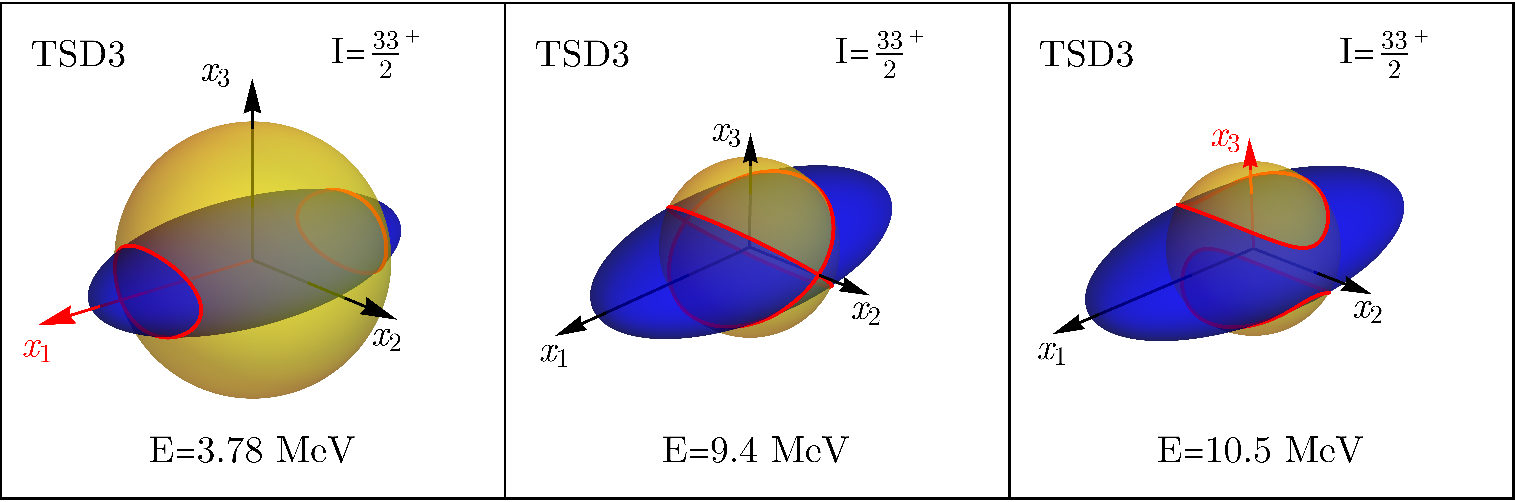
\includegraphics[width=0.99\textwidth]{Chapters/Figures/parity-partners-plots/classical-trajectory-TSD3.pdf}
    \caption{The nuclear trajectories for the state $I=33/2^+$ from TSD3 in $^{163}$Lu. The left inset shows the trajectory of the system corresponding to the real energy of this particular spin (i.e., the red ellipses that surround $x_1$). The rotational axis is marked by the red color, signifying that the nucleus wobbles around it. See text for more details.}
    \label{classical-trajectory-TSD3-plot}
\end{figure}
\begin{figure}
    \centering
    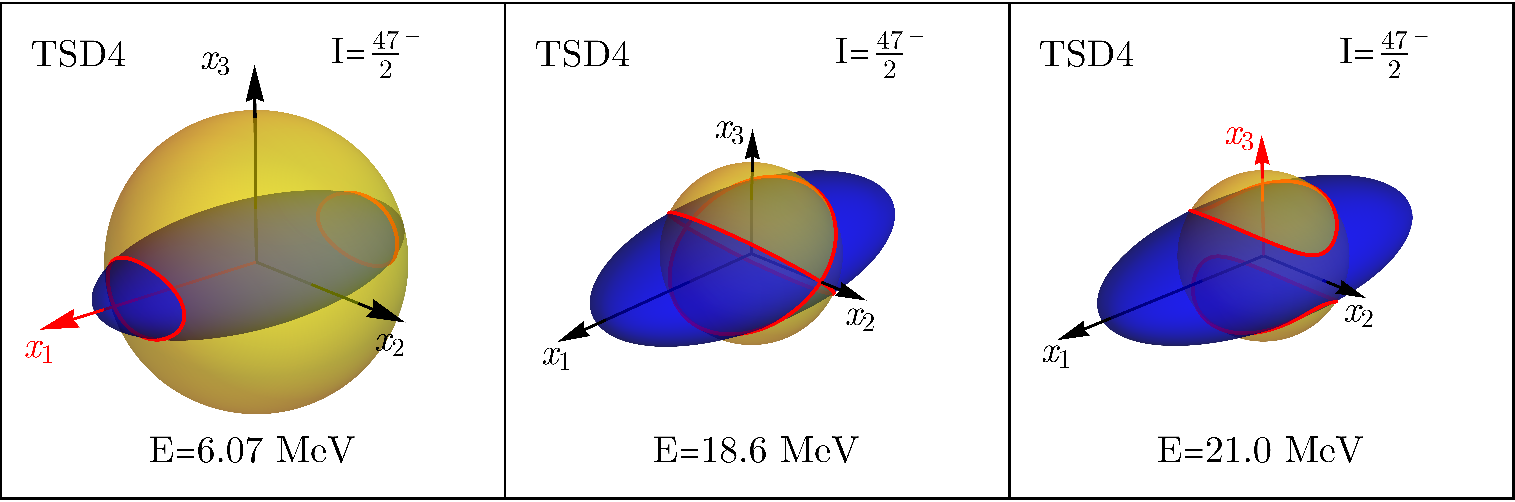
\includegraphics[width=0.99\textwidth]{Chapters/Figures/parity-partners-plots/classical-trajectory-TSD4.pdf}
    \caption{The nuclear trajectories for the state $I=47/2^+$ from TSD4 in $^{163}$Lu. The left inset shows the trajectory of the system corresponding to the real energy of this particular spin (i.e., the red ellipses that surround $x_1$). The rotational axis is marked by the red color, signifying that the nucleus wobbles around it. See text for more details.}
    \label{classical-trajectory-TSD4-plot}
\end{figure}

For low-lying states, the two orbits lie quite close to the $x_1$-axis, making the rotation more pronounced around the $x_1$ and $-x_1$ directions. As the energy increases, the precession of $\mathbf{I}$ increases as well, making the two trajectories approach each other, resulting in a \emph{tilted rotation} of the system. The tilt implies that the rotational axis is misaligned and it is moving away from its \emph{equilibrium point} \cite{poenaru2021extensive2}. Increasing the energy even further will make the two trajectories intersect with each other, marking a \emph{critical point} where the wobbling motion becomes unstable. This is represented by the middle inset throughout Figs. \ref{classical-trajectory-TSD1-plot} - \ref{classical-trajectory-TSD4-plot}. Lastly, if the energy increases beyond the critical point, a different picture emerges, where the rotational axis changes from $x_1$ to $x_3$. Such a transition is shown in the right inset of each figure, where two symmetric paths are visible along the $x_3$- and $-x_3$-directions. However, the energies at which the nucleus could undergo a change in the rotational axis are way too large for a phase transition to occur naturally in $^{163}$Lu. Concisely, the state $I=25/2^+$ from TSD1 has a real energy of about $2.6\ \text{MeV}$, while the critical value requires twice that amount. Nonetheless, this is another remarking aspect of the current formalism, showing that phase transitions between rotational modes can be identified.

Comparing the description of the wobbling motion made in the 3-dimensional space and the one from the previous subsection, both are able to pinpoint regions where phase transitions for the nuclear wobbling motion can take place. Identifying the changes in the rotational character for a triaxial nucleus was successful in each case. In addition, the geometrical analysis using the energy surface $E'$ from Eq. \ref{energy-surface-E} provides a clearer interpretation of the underlying motion, since the precession of $\mathbf{I}$ is directly related to the trajectories attained by intersecting $E'$ with the angular momentum sphere.

\section{Concluding Remarks}

In this chapter, a novel approach for the wobbling motion in odd-mass nuclei was presented, starting with the theoretical calculations and finally comparing the obtained results with the experimental data. Indeed, the idea of Signature Partner Bands firstly employed by the team in $\mathbf{W_1}$ was amended with the concept of Parity Partners, making a renormalization of the wobbling band structure and naming it $\mathbf{W_2}$ (see subsection\ref{parity-partners-renormalizaion}). It is shown that the Hamiltonian admits functions with both positive and negative parities, and thus $^{163}$Lu is considered as the testing nucleus. The renormalization of $\mathbf{W_2}$ gives a new energy spectrum of the four TSD bands, which is expressed by Eq. \ref{tsd-energies-lu163-parity-partners}. The same TDVE was applied to the states TSD1-2 and TSD4, except that herein, all four bands are obtained from the coupling of the same $i_{13/2}$ odd proton with a core of even spin states (TSD1) and odd spin states (TSD2,4). The coupling schemes are sketched in Table \ref{lu163-table-info}. Compared to the $\mathbf{W_1}$ method, here $^{163}$Lu is described by a single fitting procedure, and it consisted of minimizing the $\chi^2$-function from Eq. \ref{chi-2-fitting-function} w.r.t. the free parameters defined in \ref{fitting-parameters-p-fit}. 

The numerical results were presented in Section \ref{aw2-numerical-results}, where one obtained a very good agreement with the experimental data for the excitation energies (recall Figs. \ref{results-parity-partners-163lu-1} - \ref{results-parity-partners-163lu-2}), resulting in deviations of less than $100\ \text{keV}$ across the spectrum. The fitting parameters provided in Table \ref{lu163-parameters-parity-fitting} were also interpreted in terms of their numerical values, and compared with previous studies. The current model gives a realistic approximation of the triaxiality parameter and also the single-particle potential strength. In addition, the three moments of inertia obtained from the fit agree with the hydrodynamic model (i.e., the irrotational MOI) and Fig. \ref{w2-mois-comparison} shows this feature. The last major step in the study was to examine the average of the total Hamiltonian on the trial function adopted in $\mathbf{W_2}$. One started with the expression of the classical energy function in the minimum point $(0,I;0,j)$, which is defined in Eq. \ref{CEF-minimum-point-Tcore-Tsp}. Then, two subsequent investigations were made, namely i) finding the behavior fo $\mathcal{H}$ with respect to the polar coordinates $(\theta,\varphi)$ that are used to generate the angular momentum components (Eq. \ref{angular-momentum-polar-components}) and ii) extending the problem from 2D to 3D, by adopting the so-called energy surface. In the case $i)$, by creating contour plots in the polar plane, three minima are observed, each surrounded by closed orbits that indicate a stable motion. Beyond a critical value $\mathcal{H}_\text{critical}$, the orbits become non-localized and they now surround all three minimum points. In Fig. \ref{fig-H-unstable-sketch} the regions with stable and unstable character are sketched, and a phase transition between them is highlighted. The case $ii)$ aims at expressing $\mathcal{H}$ in terms of the cartesian components of $I$. This is achieved via Eq. \ref{constant-of-motion-E} that becomes the energy surface. Its intersection with the angular momentum sphere will point out nuclear trajectories, i.e., manifolds in the angular momentum space that show the precessional motion of the spin states belonging to the wobbling bands of $^{163}$Lu.

The 3-dimensional technique presented in the last subsection concluded with the set of Figs. \ref{classical-trajectory-TSD1-plot} - \ref{classical-trajectory-TSD4-plot}, which are very useful for getting a grasp on the inherent dynamics of the system. Certainly, through the clear dissimilarities between each nuclear phase (precession around $x_1$, criticality, and finally precession around $x_3$), one is able to understand the geometry of the rotational motion for a triaxial nucleus. The exact energy for a given spin state $I$ at which unstable wobbling occurs (the middle inset from Figs. \ref{classical-trajectory-TSD1-plot} - \ref{classical-trajectory-TSD4-plot}) was numerically determined for all four bands. Since the entire formalism is based on the dequantization of $\hat{H}$ by virtue of the variational principle and because the CEF is strictly described in terms of the canonical coordinates $(r,\varphi;f,\psi)$, the obtained trajectories can indeed be regarded as classical quantities.